\documentclass[tikz,border=8pt]{standalone}
% Shared TikZ preamble for book diagrams
% Usage: % Shared TikZ preamble for book diagrams
% Usage: % Shared TikZ preamble for book diagrams
% Usage: \input{../preamble.tex} after \documentclass

\usepackage{tikz}
\usepackage{amsmath,amssymb}

\usetikzlibrary{arrows.meta, calc, positioning, decorations.pathreplacing}

% --- Color palette ---
% Consistent across all diagrams in the book
\definecolor{basis1}{RGB}{31,119,180}    % blue: encoders, structure
\definecolor{msg}{RGB}{44,160,44}        % green: positives
\definecolor{aux}{RGB}{127,127,127}      % gray: alternatives, auxiliary
\definecolor{highlight}{RGB}{255,127,14} % orange: highlights
\definecolor{lightfill}{RGB}{230,240,255}% light blue: shaded regions

% --- Reusable styles ---
\tikzset{
  encoder/.style={draw=basis1!60, fill=lightfill, rounded corners=3pt,
    minimum width=1.0cm, minimum height=0.8cm},
  flow/.style={-{Stealth[length=5pt,width=4pt]}, line width=0.8pt},
  annotation/.style={font=\footnotesize, text=aux!80!black},
}
 after \documentclass

\usepackage{tikz}
\usepackage{amsmath,amssymb}

\usetikzlibrary{arrows.meta, calc, positioning, decorations.pathreplacing}

% --- Color palette ---
% Consistent across all diagrams in the book
\definecolor{basis1}{RGB}{31,119,180}    % blue: encoders, structure
\definecolor{msg}{RGB}{44,160,44}        % green: positives
\definecolor{aux}{RGB}{127,127,127}      % gray: alternatives, auxiliary
\definecolor{highlight}{RGB}{255,127,14} % orange: highlights
\definecolor{lightfill}{RGB}{230,240,255}% light blue: shaded regions

% --- Reusable styles ---
\tikzset{
  encoder/.style={draw=basis1!60, fill=lightfill, rounded corners=3pt,
    minimum width=1.0cm, minimum height=0.8cm},
  flow/.style={-{Stealth[length=5pt,width=4pt]}, line width=0.8pt},
  annotation/.style={font=\footnotesize, text=aux!80!black},
}
 after \documentclass

\usepackage{tikz}
\usepackage{amsmath,amssymb}

\usetikzlibrary{arrows.meta, calc, positioning, decorations.pathreplacing}

% --- Color palette ---
% Consistent across all diagrams in the book
\definecolor{basis1}{RGB}{31,119,180}    % blue: encoders, structure
\definecolor{msg}{RGB}{44,160,44}        % green: positives
\definecolor{aux}{RGB}{127,127,127}      % gray: alternatives, auxiliary
\definecolor{highlight}{RGB}{255,127,14} % orange: highlights
\definecolor{lightfill}{RGB}{230,240,255}% light blue: shaded regions

% --- Reusable styles ---
\tikzset{
  encoder/.style={draw=basis1!60, fill=lightfill, rounded corners=3pt,
    minimum width=1.0cm, minimum height=0.8cm},
  flow/.style={-{Stealth[length=5pt,width=4pt]}, line width=0.8pt},
  annotation/.style={font=\footnotesize, text=aux!80!black},
}


\begin{document}
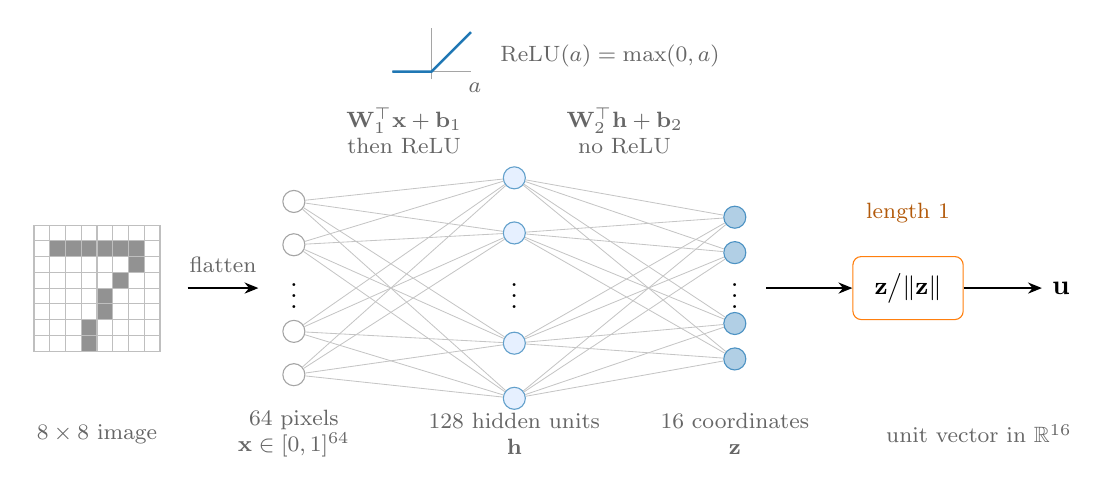
\begin{tikzpicture}[
  unit/.style={circle, draw=aux!70, fill=white, minimum size=0.28cm, inner sep=0pt},
  hid/.style={unit, draw=basis1!70, fill=lightfill},
  outu/.style={unit, draw=basis1!80, fill=basis1!35},
  wire/.style={aux!45, line width=0.3pt},
  pixel/.style={draw=aux!50, minimum size=0.2cm, inner sep=0pt},
]

% === Input image: 8x8 pixels, a drawn digit 7, centred on the axis of the layers ===
\begin{scope}[yshift=0.7cm]
\foreach \r in {0,...,7}{
  \foreach \c in {0,...,7}{
    \node[pixel, fill=white] at ({\c*0.2},{-\r*0.2}) {};
  }
}
\foreach \r/\c in {1/1,1/2,1/3,1/4,1/5,1/6, 2/6, 3/5, 4/4, 5/4, 6/3, 7/3}{
  \node[pixel, fill=aux!85] at ({\c*0.2},{-\r*0.2}) {};
}
\end{scope}
\node[annotation] at (0.7,-1.85) {$8\times 8$ image};

% === Layers: columns of units, the middle unit stands for the omitted ones ===
\def\xin{3.2}
\def\xhid{6.0}
\def\xout{8.8}
\foreach \k/\y in {1/1.1,2/0.55,3/-0.55,4/-1.1}{ \node[unit] (i\k) at (\xin,\y) {}; }
\foreach \k/\y in {1/1.4,2/0.7,3/-0.7,4/-1.4}{ \node[hid] (h\k) at (\xhid,\y) {}; }
\foreach \k/\y in {1/0.9,2/0.45,3/-0.45,4/-0.9}{ \node[outu] (o\k) at (\xout,\y) {}; }
\foreach \x in {\xin,\xhid,\xout}{ \node at (\x,0) {$\vdots$}; }

% === Fully connected wires ===
\foreach \a in {1,2,3,4}{
  \foreach \b in {1,2,3,4}{ \draw[wire] (i\a) -- (h\b); \draw[wire] (h\a) -- (o\b); }
}

% === Flatten arrow ===
\draw[flow] (1.85,0) -- (2.75,0);
\node[annotation] at (2.3,0.3) {flatten};

% === Normalization and output ===
\node[draw=highlight, rounded corners=3pt, minimum width=1.4cm, minimum height=0.8cm, align=center, font=\small]
  (norm) at (11.0,0) {$\mathbf{z}\big/\lVert\mathbf{z}\rVert$};
\draw[flow] (9.2,0) -- (norm);
\draw[flow] (norm) -- (12.7,0) node[right] {$\mathbf{u}$};

% === Labels above the layers ===
\node[annotation, align=center] at (4.6,2.0) {$\mathbf{W}_1^\top\mathbf{x}+\mathbf{b}_1$\\then ReLU};
\node[annotation, align=center] at (7.4,2.0) {$\mathbf{W}_2^\top\mathbf{h}+\mathbf{b}_2$\\no ReLU};
\node[annotation, align=center, text=highlight!70!black] at (11.0,0.95) {length 1};

% === ReLU defined: graph of max(0,a) ===
\begin{scope}[shift={(4.95,2.75)}]
  \draw[aux!70, line width=0.4pt] (-0.5,0) -- (0.5,0);
  \draw[aux!70, line width=0.4pt] (0,-0.1) -- (0,0.55);
  \draw[basis1, line width=0.9pt] (-0.5,0) -- (0,0) -- (0.5,0.5);
  \node[annotation, anchor=west] at (0.75,0.2) {$\mathrm{ReLU}(a)=\max(0,a)$};
  \node[annotation] at (0.55,-0.2) {$a$};
\end{scope}

% === Labels below the layers ===
\node[annotation, align=center] at (\xin,-1.85) {64 pixels\\$\mathbf{x}\in[0,1]^{64}$};
\node[annotation, align=center] at (\xhid,-1.85) {128 hidden units\\$\mathbf{h}$};
\node[annotation, align=center] at (\xout,-1.85) {16 coordinates\\$\mathbf{z}$};
\node[annotation, align=center] at (11.9,-1.85) {unit vector in $\mathbb{R}^{16}$};

\end{tikzpicture}
\end{document}
